\lettrine{T}{his appendix chapter} includes some additional information about the models I have run. I include this to discuss some of the notable features and challenges to the models, and how I account for this.

\section{Residuals}
I here display the residual plot of Model 2.5 in Table \ref{tab:h2}. The residuals are quite similarly distributed in all the main plots. We can see a very distinct shape to the plot, but there are two important ting to note, ant that is: one, the model is unbiased, and two, this problem of heteroscedasticity can be solved by using clustered standard errors.

\begin{figure}[H]
    \centering
    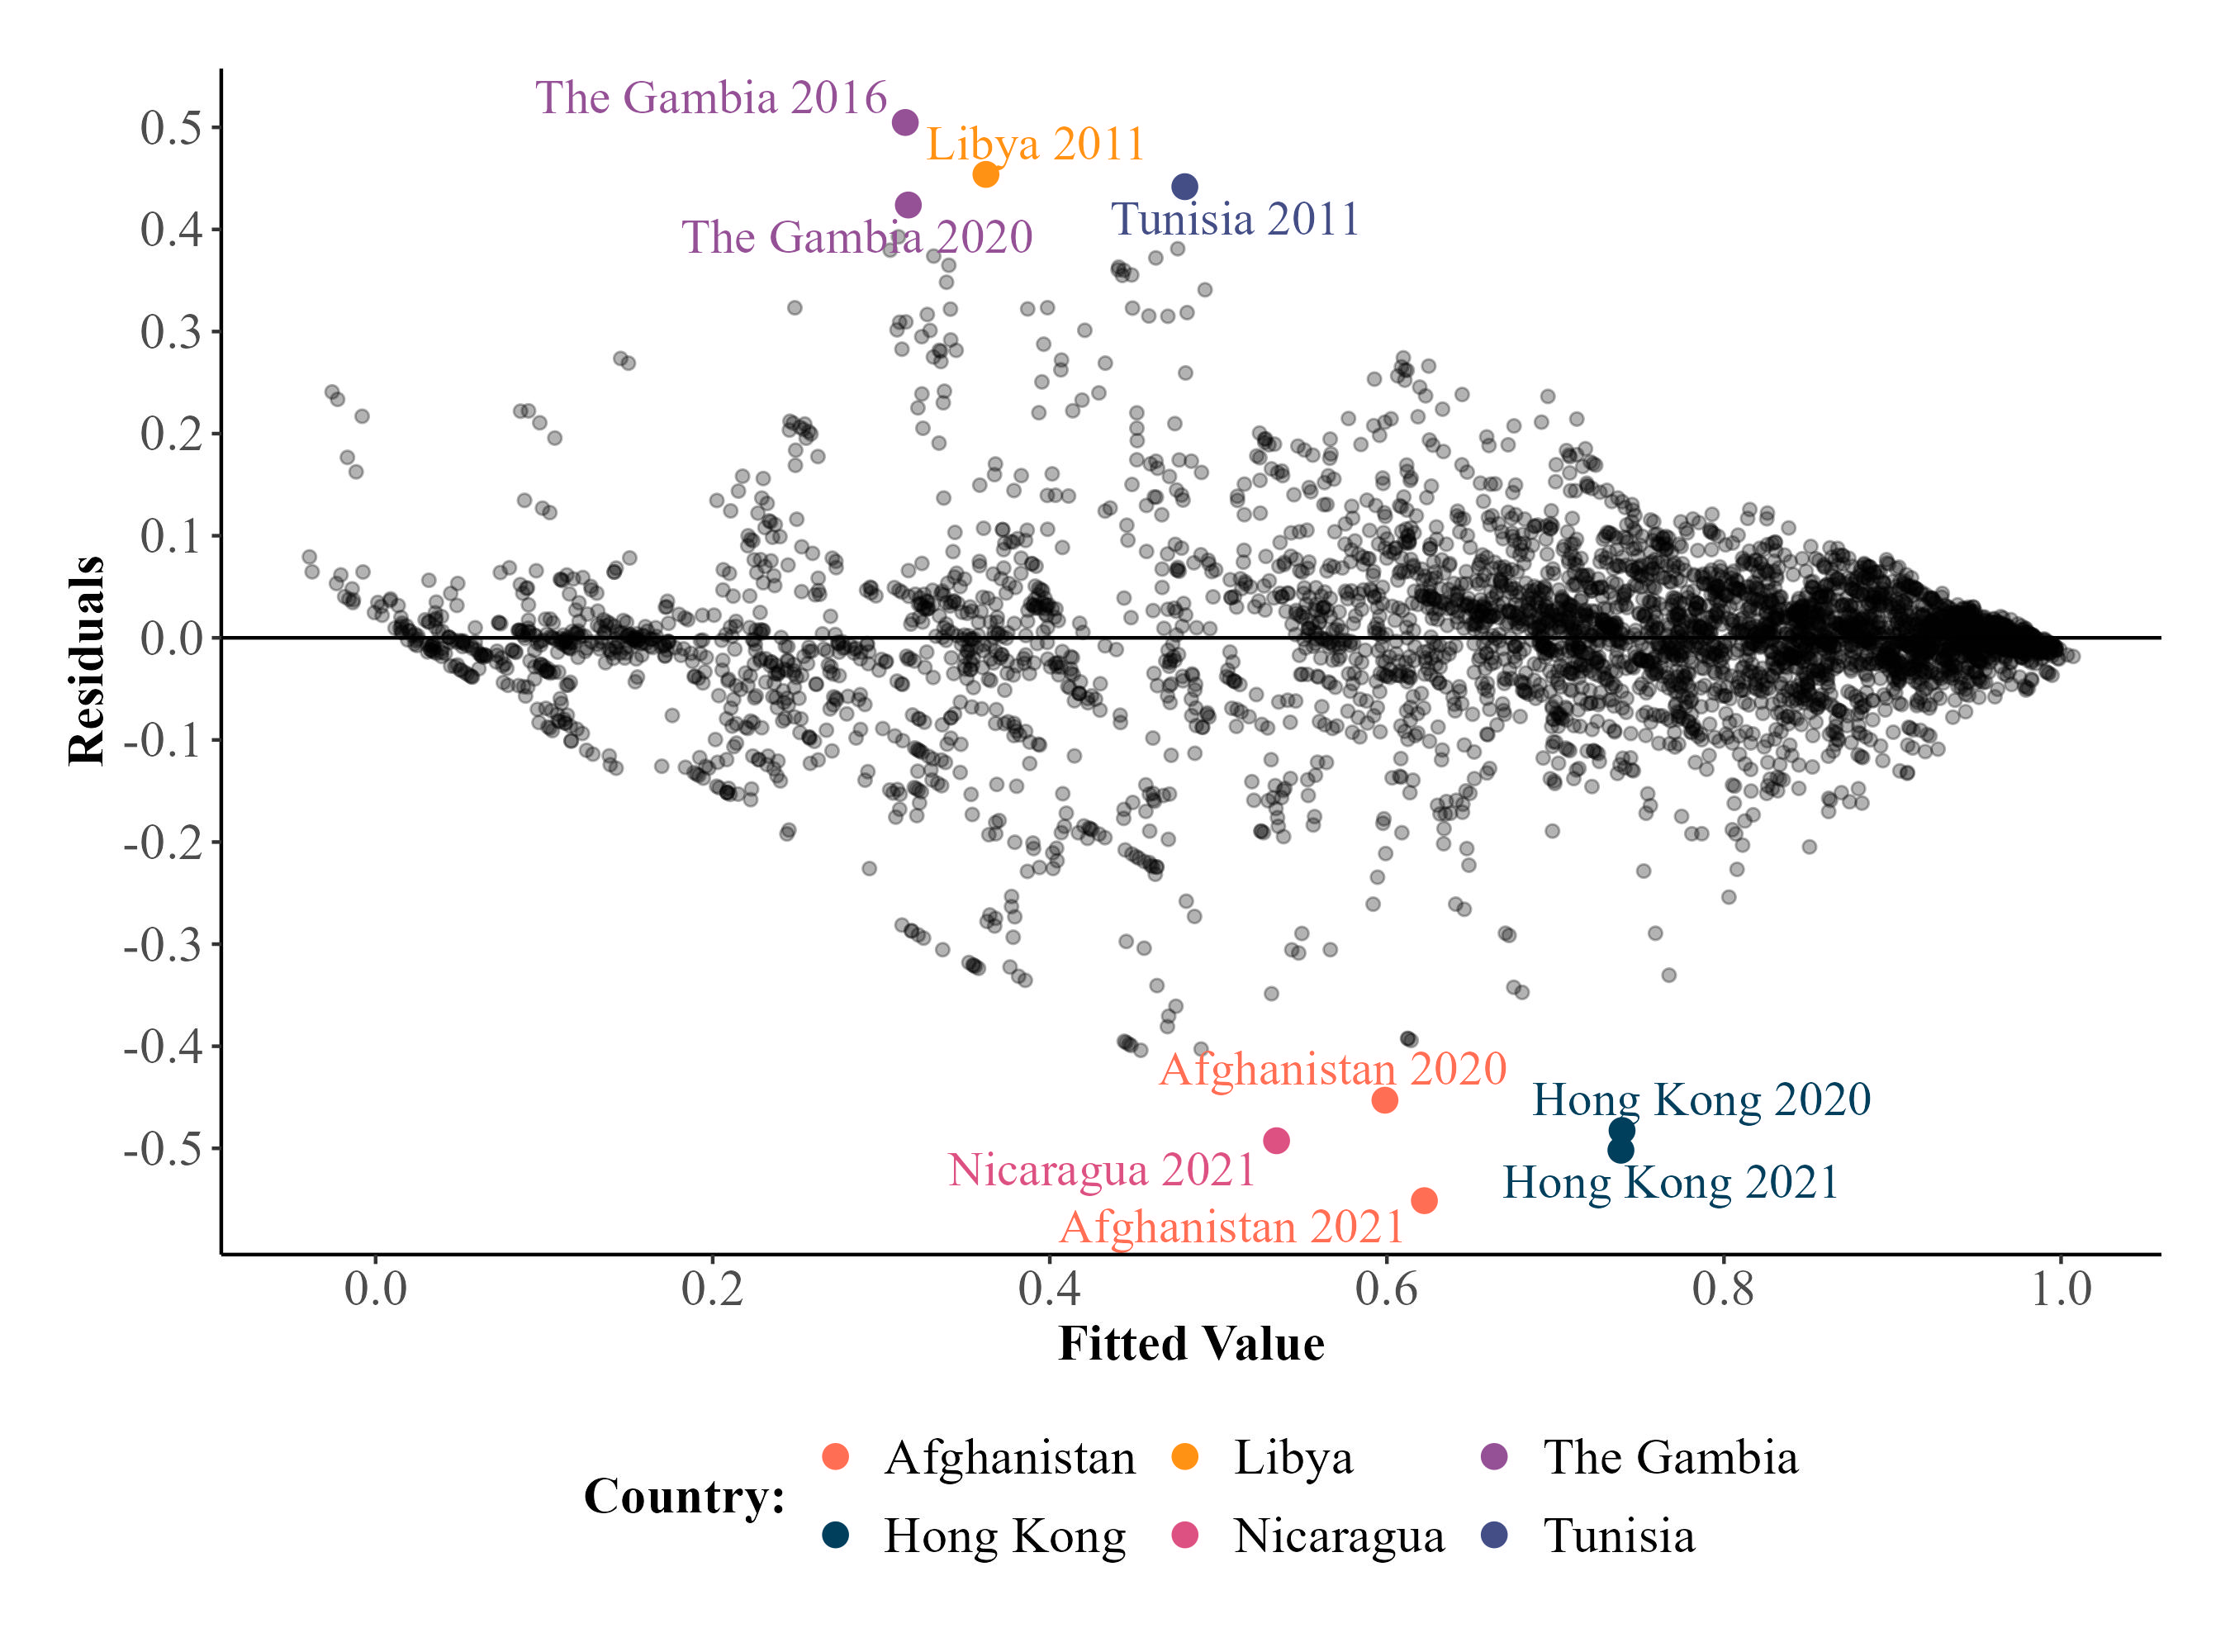
\includegraphics[width=.9\linewidth]{graphics/residuals.jpeg}
    \caption{Residual plot for Model 2.5}
    \label{fig:residuals}
\end{figure}